%
%
%Introduction goes here...
%
%
%%----------------------------------------------------------------------
%\section{First Section} 
%\label{sec:SECTION1NAME}
%
%Text of section 1 goes here... \\
%
%This is to insert a table \\
%
%\begin{table}
%\begin{center}
%\begin{tabular}{|l|c|}
%\hline
%Method & Frobnability \\
%\hline\hline
%Theirs & Frumpy \\
%Yours & Frobbly \\
%Ours & Makes one's heart Frob\\
%\hline
%\end{tabular}
%\end{center}
%\caption{Results.   Ours is better.}
%\end{table}
%
%This is to insert a figure \\
%
%\begin{figure}[h]
%\centering
%
\includegraphics[height=2cm,width=0.2\linewidth]{figures/iiit.eps}
%\caption{Analysis of our method}
%\label{}
%\end{figure}
%
%
%
%%----------------------------------------------------------------------
%\section{Second Section} 
%\label{sec:SECTION2NAME}
%
%Text of section 2 goes here... \\
%
%{\bf Few suggestions}
%
%%-------------------------------
%\subsection{Mathematics}
%
%Please number all of your sections and displayed equations.  It is
%important for readers to be able to refer to any particular equation.  Just
%because you didn't refer to it in the text doesn't mean some future reader
%might not need to refer to it.  It is cumbersome to have to use
%circumlocutions like ``the equation second from the top of page 3 column
%1''.  (Note that the ruler will not be present in the final copy, so is not
%an alternative to equation numbers).  All authors will benefit from reading
%Mermin's description of how to write mathematics (see math.pdf).
%
%
%%------------------------------
%\subsection{Footnotes}
%
%Please use footnotes\footnote {This is what a footnote looks like.  It
%often distracts the reader from the main flow of the argument.} sparingly.
%Indeed, try to avoid footnotes altogether and include necessary peripheral
%observations in 
%the text (within parentheses, if you prefer, as in this sentence).  If you
%wish to use a footnote, place it at the bottom of the column on the page on
%which it is referenced. Use Times 8-point type, single-spaced.
%
%%--------------------------------
%\subsection{References}
%
%List and number all bibliographical references in 9-point Times,
%single-spaced, at the end of your paper. When referenced in the text,
%enclose the citation number in square brackets, for
%example~\cite{Authors06}.  Where appropriate, include the name(s) of
%editors of referenced books.
%
%%--------------------------------
%\subsection{Illustrations, graphs, and photographs}
%
%All graphics should be centered.  Please ensure that any point you wish to
%make is resolvable in a printed copy of the paper.  Resize fonts in figures
%to match the font in the body text, and choose line widths which render
%effectively in print.  Many readers (and reviewers), even of an electronic
%copy, will choose to print your paper in order to read it.  You cannot
%insist that they do otherwise, and therefore must not assume that they can
%zoom in to see tiny details on a graphic.
%
%%---------------------------------
%\subsection{Color}
%
%Color is valuable, and will be visible to readers of the electronic copy.
%However ensure that, when printed on a monochrome printer, no important
%information is lost by the conversion to grayscale.
%
%
%For more suggestions to improve your document, see preparationGuide.pdf

We live in a world which is increasingly becoming multilingual and at the same time, increasingly automated. The amount of multimedia and captured data are rapidly increasing and stored in digital format. These data also includes multilingual document images, scene images and videos containing text which can play a crucial role in understanding the document images as well as scene/video images. 
For example, there are many museums which store images of all old and fragile documents which are of importance to historians and other researchers for analysis and archival purposes. While touring in foreign countries, we may not what all the sign boards say. 

Several Optical Character Recognition (\textsc{ocr}) tools and systems are used to convert different types of documents, such as scanned document images, \textsc{pdf} files or images captured by a digital camera into editable and retrievable data. Given a document image or scene images, a general \textsc{ocr} will do following tasks:
\begin{itemize}
\item \textbf{Preprocessor:} It typically includes binarization and noise cleaning followed by skew detection and correction. This step is required by the subsequent steps which works best with binary images. Popular binarization techniques include Otsu method for document images and ~\cite{Authors06b} for texts in scene or video images.
\item \textbf{Segmentation:} Once the documents are processed, a layout engine is used to extract the structure of the documents. Several document exists which can be used to find the text area, graphics area, table area and other document elements in the document. Words and lines are then segmented from the text area using connected component analysis. The resulting symbols are then recognized by the recognition tool.
\item \textbf{Feature Extraction:} Local and global features are then extracted from the symbols extracted above. Some commonly used features include \textsc{hog}, \textsc{sift}, profile based features, appearance based features etc.
\item \textbf{Classification:} Features extracted above is then given as input to off-the-self classifiers to classify the input features to one of the possible output labels. For linearly separable features, linear Support Vector Machines (\textsc{svm}) is used else, classifiers like Neural Networks. \textsc{hmm}s, Random Forests, etc.
\item \textbf{Post-processor:} Output obtained from the classifier is then corrected by dictionary based language models.
\end{itemize}

\begin{figure*}[h]
\centering 
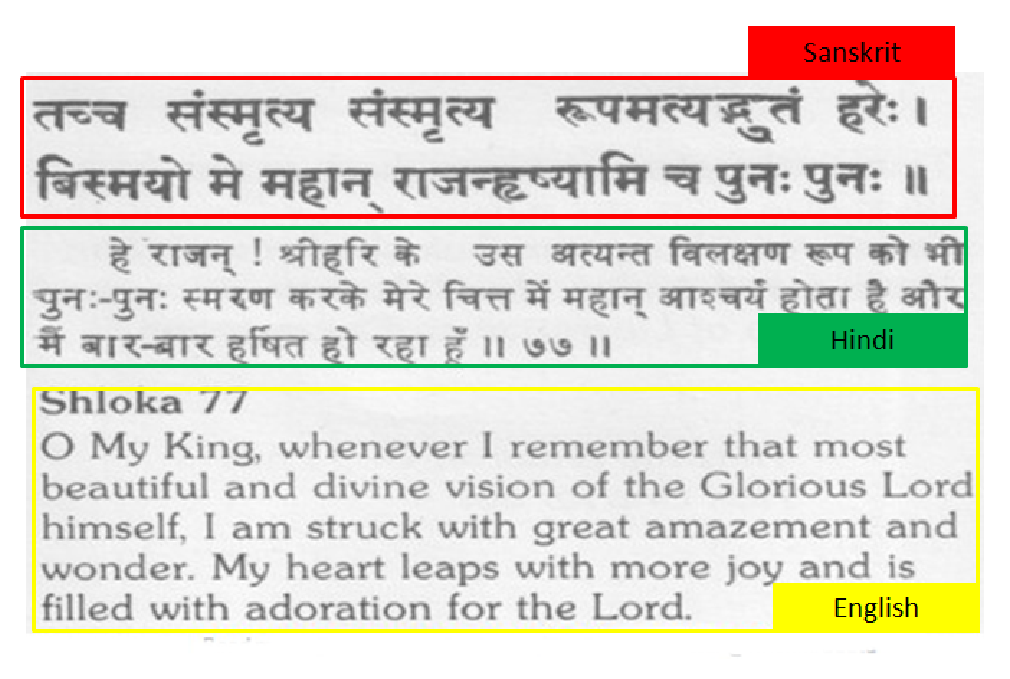
\includegraphics[scale=0.5]{/home/ajeet/Dropbox/Singh_Thesis/figures/multilingual.eps}
\caption{A sample document image containing three languages: Sanskrit, Hindi and English. When an individual English/Hindi \textsc{ocr} will be run on this document, the recognition output will not be accurate. But, when a multilingual \textsc{ocr} containing a script identification module will be able to recognize the inherent text with high accuracy.}
\label{fig:motFig}
\end{figure*}

It can be seen from the above \textsc{ocr} process, all the existing \textsc{ocr} systems makes an assumption that the language of the text document and scene/video images is known beforehand.  Individual OCR tools have been developed to deal best with only one specific language. A Hindi OCR package will deal very well with Hindi, and may be able to cope possibly with some other Devanagari alphabet languages such as Marathi or Gujarati. It will not, however, be very helpful if given a Telugu or Tamil document to process. As shown in Figure.~\ref{fig:motFig}, the document, which contains text from three different scripts, will not be correctly recognized with an individual \textsc{ocr} without a manual intervention. In an automated environment such document processing systems would clearly need human intervention to select the appropriate \textsc{ocr} package, which is obviously not desirable. A \textit{pre}-\textsc{ocr} language or script identification system would enable the correct \textsc{ocr} system to be selected in order to achieve the best character interpretation of the document. This area has widely researched to date with its growing importance to the document image processing community and the progression towards the ``paperless office".

Script identification in printed and handwritten document images is a highly researched problem. Contrary to the scanned and handwritten images, script identification in scene images poses several problems. Also, processing a scene-image is pretty difficult task than that of document images due to following:

\begin{itemize}
\item \textbf{Lack of context}. Scene text often appears as a single word or a group of words, and applying larger sentence or paragraph level context is hard. 
\item \textbf{Complex background}. Scene text come with highly complex natural scene background, on
the other hand document images often contain predominantly text.
\item \textbf{Quality of image.} The quality of the image will directly affect the identification accuracy. As scene texts are often captured under uncontrolled environments, the difficulties in identification may be caused by several factors such as low resolutions, noises and illumination changes.
\item \textbf{Similarity in scripts.} Some scripts/languages have relatively minor differences \textit{e.g.} Hindi, Gujarati and Bangla. These languages share a subset of characters that have exactly the same shapes. Distinguishing them relies on special characters or character components, and is fine-grained classification problem.
\item \textbf{Variations.} Text images have arbitrary aspect ratios, since text strings have arbitrarily lengths, ruling out some image classification methods that only operate font-sized inputs. Scene text images often contains stylish fonts to attract the viewers and do not easily generalize to the training data.
\end{itemize}

\begin{figure}
\centering
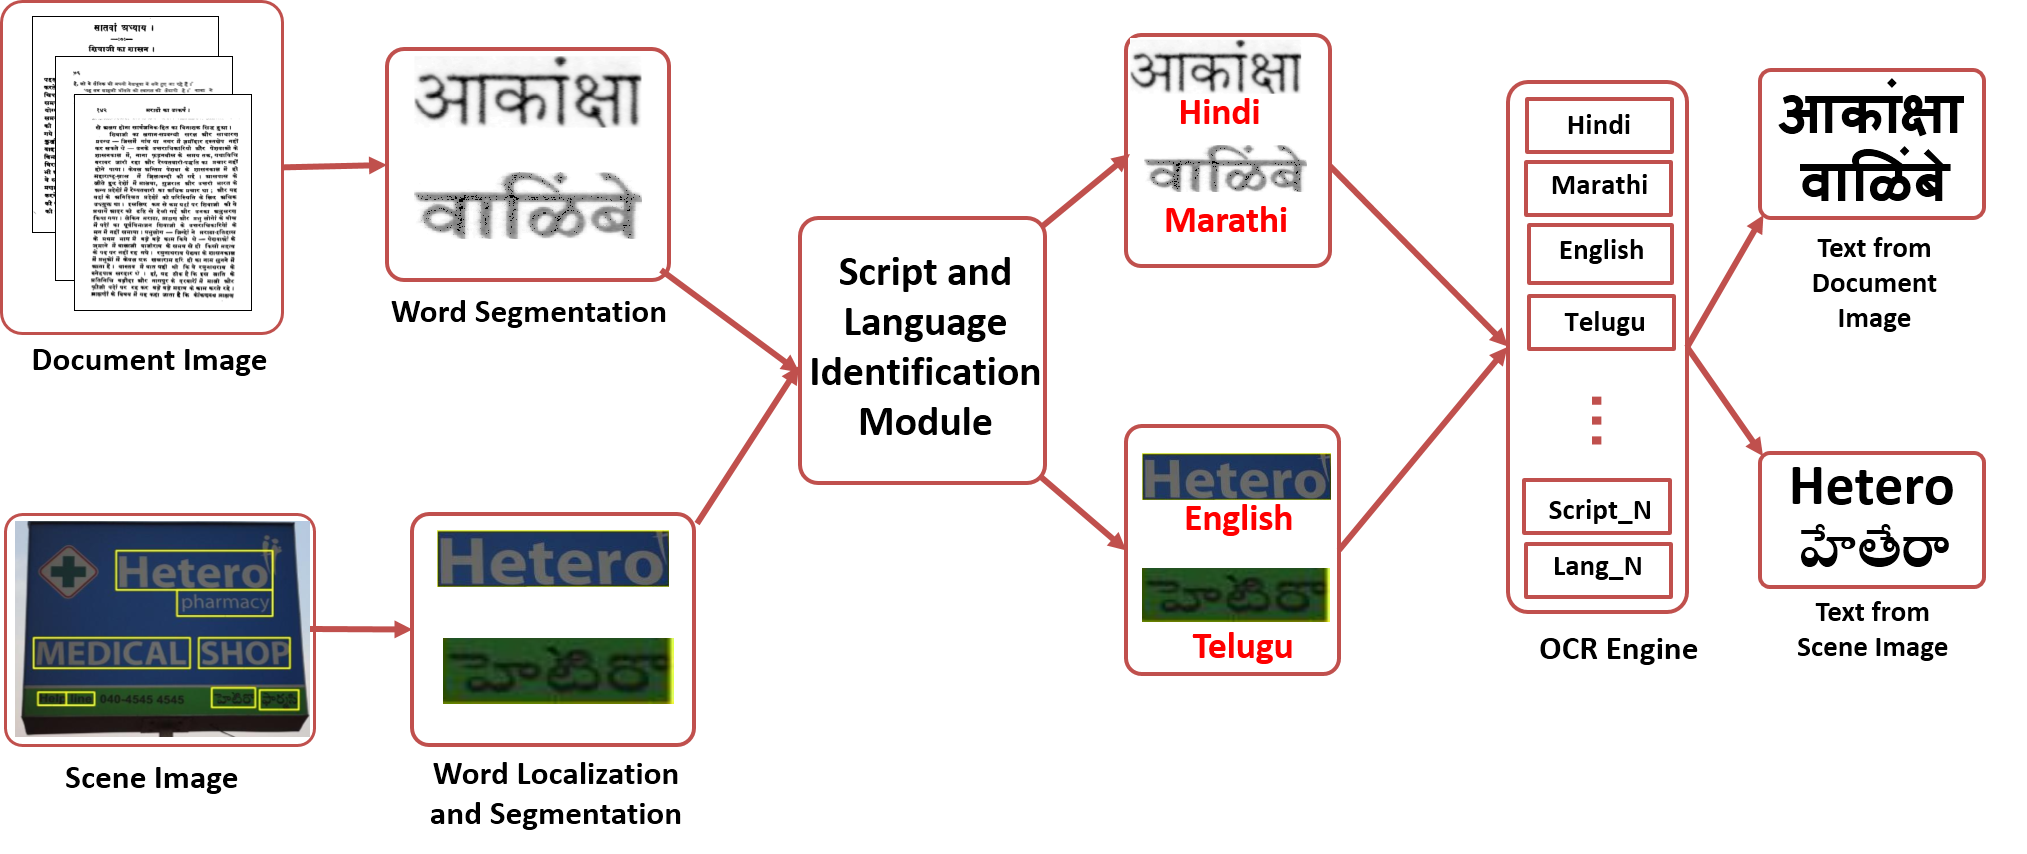
\includegraphics[scale=0.45]{figures/motivationScript.png}
\caption{ In order to move towards a ``paperless office", there are million of documents in several scripts and languages to be digitized. But due to the limitation of existing \textsc{ocr} systems, the inherent script and language of the documents should be known beforehand. Hence, a script identification module is added in \textsc{ocr} system which will identify the scripts and language at word or line level before passing it to corresponding scripts/language \textsc{ocr}.}
\label{fig:motivation}
\end{figure}

\section{Prior Art}
\label{sec:prior}

Script and language identification is highly researched area in document image analysis community. There have been several methods and approaches which deals with the script and language identification at page, line or word level. Although there are many research related to script identification at all the levels. But there is a dearth in research on language identification beyond document level. We describe the several approaches in following paragraphs which has been used in the past for the script and language identification at aforementioned levels.
\\
\


\noindent\textbf{Text Symbol based Approach:} Hochberg \textit{et al.} present a method for automatically identifying the script of a binarized document using cluster-based text symbol templates. Text symbols are rescaled to $30\times 30$ pixels. Symbols are grouped into clusters based on Hamming distances. The centroid of the clusters will act as template which will be used to calculate the distance score with test image. The script template with which distance score is low is then allotted to the test image. Note that, a distance score of the test image is calculated with all the script templates. This method is, however, prone to misclassification due to variations in fonts and is not suitable for low resolution images.
\\
\
%\noindent\textbf{Projection Profiles:} Wood \textit{et al.} present some observations about the characteristics of various scripts, with particular reference to the effect such characteristics have on the horizontal and vertical projections of the document images. The method would not require any   


\noindent\textbf{Upward Concavities:} Spitz proposes a method for distinguishing between Asian and European languages by examining the upward concavities of connected components. The upward concavities is shown to be markedly different between the languages aforementioned. Gross or document level script identification is performed by analyzing the variance of the distribution. For Asian languages such as Chinese, Japanese and Korean, an optical density function is computed whereby the total number of black pixels  in each character is tabulated in reading across the text. Study of the distributions of these optical density shows distinct differences amongst the Asian languages. Character shape codes relate to the dimensions of characters rather than the actual characters themselves. Language identification of several Roman alphabet languages is performed by statistical analysis of frequent combinations of character shape codes in the languages investigated. 
\\ 
\ 


\noindent\textbf{Texture Based approach:} 
Global approaches generally refer to the texture of the documents, line or word. These textures are complex visual pattern composed of sub-patterns. These textures can be used to measure the periodicity of the image. These textures produces variations in character density and stroke orientation. Gabor filters act as good model for texture classification~\cite{Shijian08}. A multichannel gabor filter has been employed which requires an $N\times N$ pixel as input, orientation and frequencies. Then a rotational invariant texture features were computed.
\\
\


\noindent\textbf{Neural Networks: } Lee and Kim use a self-organizing neural network in order to determine not the script of whole document but the individual characters within the document~\cite{}. After an initial character shape normalization. Zero, first, second order features are calculated using a Mesh feature system, overlapping contour direction codes~\cite{}. There are then two classification stages, a coarse classifier, followed by a fine classifier which classifies the characters in the mixed groups and presumably performs actual character identification. In recent there have been an efforts to use the discriminative features learned using Convolutional Neural Networks (\textsc{CNN}) for multi-script recognition~\cite{Rashid10}. These features are automatically extracted and learned at connected component level of the document image.
\\
\


The approaches mentioned above mainly deal at script level identification. But, when the inherent script of document images are same, visual features are hard to separate between different languages, especially when the identification is required at word level. This problem is described as language identification in document images. There are many attempts in the past in textual domain to separate the languages using statistics(\textit{e.g.} \textit{n}-gram probabilities of characters. In image domain, language identification is attempted at page level or paragraph level in the past. There have some methods proposed which
categorizes the characters based on a number of character shape features such as character ascenders and descenders. For example, ~\citep{Spitz97} group the character images into a small set of categories first. Then, based on the classification results, each word image is converted into a word shape token. Latin-based languages are finally determined according to the frequency of a single word ~\cite{Spitz97}, word pair and word trigram. Shijian and Tan ~\cite{Shijian08} combined the script and language identification using a document vectorization framework. They convert document into vertical cut vector based on the number and positions of vertical cut to capture the shape of the word directly.

\section{Goals of thesis}
This thesis addresses the problem of script and language identification in scanned document images as well as in the camera captured wild images.  The major goals of thesis are, i) Developing a simple and effective solution for script identification in the wild and ii) Script and language identification in document images at word and line level for the multi-lingual documents using deep learning, specifically Recurrent Neural Networks (\textsc{RNN}). Moreover, the scene text recognition in Indian languages is recently growing, many of the datasets for this problem are either very small or not very challenging for real scenario, hence as a part of this thesis we also introduce and benchmark Indian Language scene text datasets.


\section{Major Contributions}
This thesis has follwing major contributions to the area:

\begin{enumerate}
\item \textbf{Script Identification in Wild.} We first proposed an approach for automatically identifying the script of the text localized on the scene images Chapter ~\ref{ch:chap3}. This approach is inspired by the advancements  in mid-level stroke-based features. The scene-text are then represented with these stroke-based features, and then we use an off-the-self classifier to identify the script of the text image.
\item \textbf{Script and Language Identification using Recurrent Neural Networks.} We investigate the utility of recurrent neural networks for script and language identification (Chapter ~\ref{ch:chap4}). In this we argue that one can predict the script and language with minimal evidence (e.g. given only a word or a line) very accurately with the help of pre-trained \textsc{rnn}. We propose a simple and generic solution for the task of script and language identification which do not require any special tuning.
\item \textbf{Datasets}. We also a introduce a Indian Language Scene Text (\textsc{ILST}) dataset which is a comprehensive dataset for Indian language scene text containing six scripts commonly used in India, namely Telugu, Tamil, Malayalam, Kannada, Hindi and English. The dataset contains 500 scene images with more than 4000 words. It can be used for following tasks: text localization, recognition, script identification. In this work we use this dataset for two tasks- cropped word script identification and text localization with script identification (i.e., end-to-end pipeline).
\end{enumerate}

\section{Thesis Outline}
\begin{itemize}
\item \textbf{Chapter-2.} In this chapter, we provide the necessary background for this thesis and briefly summarize the aspects of recurrent neural networks, bag-of-strokes directly relevant to the  works as follows.
\item \textbf{Chapter-3.} This chapter focuses on end-to-end script identification in the wild using mid-level bag-of-strokes features. The proposed method is compared with recently organized \textsc{cvsi}~\cite{ICDARcomp11} and also a new dataset for Indian Languages is introduced and benchmarked.
\item \textbf{Chapter-4.} This chapter focuses on usage of deep learning methods such as Recurrent Neural Networks for script and language identification in document image with minimal evidence (only words and lines). The proposed method have been tested on 55K documents from 15 different scripts and languages.
\item \textbf{Chapter-5.} This chapter summarizes our work, comparisons and impacts of the work. Here we also discuss the final version of thesis.
\end{itemize}

